% QuizForge Backend Documentation - Part 2: Data Models
\documentclass[12pt,a4paper]{report}

% Packages
\usepackage[utf8]{inputenc}
\usepackage[T1]{fontenc}
\usepackage{geometry}
\usepackage{graphicx}
\usepackage{tikz}
\usetikzlibrary{shapes.multipart, positioning, arrows.meta, calc}
\usepackage{listings}
\usepackage{xcolor}
\usepackage{hyperref}
\usepackage{tcolorbox}
\usepackage{fancyhdr}
\usepackage{titlesec}
\usepackage{longtable}
\usepackage{array}
\usepackage{booktabs}
\usepackage{enumitem}
\usepackage{pdflscape}

% Page geometry
\geometry{
    a4paper,
    left=25mm,
    right=25mm,
    top=30mm,
    bottom=30mm
}

% Colors
\definecolor{codegreen}{rgb}{0,0.6,0}
\definecolor{codegray}{rgb}{0.5,0.5,0.5}
\definecolor{codepurple}{rgb}{0.58,0,0.82}
\definecolor{backcolour}{rgb}{0.95,0.95,0.92}
\definecolor{javakey}{rgb}{0.5,0,0.35}

% Code listing style
\lstdefinestyle{javastyle}{
    backgroundcolor=\color{backcolour},
    commentstyle=\color{codegreen},
    keywordstyle=\color{javakey}\bfseries,
    numberstyle=\tiny\color{codegray},
    stringstyle=\color{codepurple},
    basicstyle=\ttfamily\footnotesize,
    breakatwhitespace=false,
    breaklines=true,
    captionpos=b,
    keepspaces=true,
    numbers=left,
    numbersep=5pt,
    showspaces=false,
    showstringspaces=false,
    showtabs=false,
    tabsize=2,
    frame=single,
    language=Java
}

\lstset{style=javastyle}

% Hyperref setup
\hypersetup{
    colorlinks=true,
    linkcolor=blue,
    filecolor=magenta,
    urlcolor=cyan,
    pdftitle={QuizForge Backend Documentation - Part 2},
    pdfauthor={System Documentation},
    pdfsubject={Data Models and Repositories},
}

% Headers and footers
\pagestyle{fancy}
\fancyhf{}
\fancyhead[L]{\leftmark}
\fancyhead[R]{QuizForge Backend - Part 2}
\fancyfoot[C]{\thepage}

% Title formatting
\titleformat{\chapter}[display]
{\normalfont\huge\bfseries}{\chaptertitlename\ \thechapter}{20pt}{\Huge}

% Document metadata
\title{%
    \Huge\textbf{QuizForge} \\
    \Large Complete Backend Documentation \\
    \large Part 2: Data Models \& Repositories \\
    \normalsize Version 1.0.0
}
\author{Technical Documentation}
\date{\today}

\begin{document}

% Title page
\maketitle
\tableofcontents
\newpage

% Include chapters for Part 2
% Chapter 3: Models (Part 1)
\chapter{Data Models (JPA Entities)}

\section{Overview}

The application uses six JPA entities that map to PostgreSQL database tables. These entities form the core data model and define the relationships between different domain objects.

\section{User Entity}

\subsection{Purpose}
The \texttt{User} entity represents system users with role-based access control. It supports two roles: ADMIN and CANDIDATE.

\subsection{Complete Source Code}

\begin{lstlisting}[caption=User.java - Complete Implementation]
package com.quizforge.model;

import jakarta.persistence.*;
import lombok.AllArgsConstructor;
import lombok.Data;
import lombok.NoArgsConstructor;

import java.time.LocalDateTime;

@Entity
@Table(name = ''users'')
@Data
@NoArgsConstructor
@AllArgsConstructor
public class User {
    @Id
    @GeneratedValue(strategy = GenerationType.IDENTITY)
    private Long id;

    @Column(nullable = false, unique = true)
    private String email;

    @Column(nullable = false)
    private String password;

    @Column(nullable = false)
    private String name;

    @Enumerated(EnumType.STRING)
    @Column(nullable = false)
    private Role role;

    @Column(name = ''created_at'', nullable = false, updatable = false)
    private LocalDateTime createdAt;

    @PrePersist
    protected void onCreate() {
        createdAt = LocalDateTime.now();
    }

    public enum Role {
        ADMIN, CANDIDATE
    }
}
\end{lstlisting}

\subsection{Line-by-Line Explanation}

\begin{itemize}[leftmargin=*]
    \item \textbf{Line 1-7:} Package declaration and imports
    \begin{itemize}
        \item \texttt{jakarta.persistence.*}: JPA annotations for entity mapping
        \item \texttt{lombok.*}: Code generation annotations
        \item \texttt{java.time.LocalDateTime}: For timestamp fields
    \end{itemize}
    
    \item \textbf{Line 9: @Entity}
    \begin{itemize}
        \item Marks this class as a JPA entity
        \item Will be managed by EntityManager
        \item Participates in persistence lifecycle
    \end{itemize}
    
    \item \textbf{Line 10: @Table(name = ''users'')}
    \begin{itemize}
        \item Maps entity to ''users'' table in database
        \item If omitted, table name would default to ''User''
        \item ''users'' avoids potential reserved word conflicts
    \end{itemize}
    
    \item \textbf{Line 11: @Data}
    \begin{itemize}
        \item Lombok annotation generating: getters, setters, toString(), equals(), hashCode()
        \item Reduces boilerplate code significantly
        \item Generated at compile time
    \end{itemize}
    
    \item \textbf{Line 12-13: @NoArgsConstructor, @AllArgsConstructor}
    \begin{itemize}
        \item Generate no-args and all-args constructors
        \item Required by JPA for entity instantiation
        \item Useful for creating instances in application code
    \end{itemize}
    
    \item \textbf{Line 15-17: Primary Key}
    \begin{itemize}
        \item \texttt{@Id}: Marks field as primary key
        \item \texttt{@GeneratedValue(strategy = GenerationType.IDENTITY)}: Auto-increment by database
        \item \texttt{Long id}: Surrogate key, nullable until persisted
    \end{itemize}
    
    \item \textbf{Line 19-20: Email Field}
    \begin{itemize}
        \item \texttt{nullable = false}: NOT NULL constraint in database
        \item \texttt{unique = true}: UNIQUE constraint, enforces no duplicates
        \item Used as username for authentication
    \end{itemize}
    
    \item \textbf{Line 22-23: Password Field}
    \begin{itemize}
        \item Stores user password
        \item Should be encrypted (BCrypt) in production
        \item Currently simplified for demo purposes
    \end{itemize}
    
    \item \textbf{Line 25-26: Name Field}
    \begin{itemize}
        \item Display name for the user
        \item Required field (nullable = false)
    \end{itemize}
    
    \item \textbf{Line 28-30: Role Field (Enum)}
    \begin{itemize}
        \item \texttt{@Enumerated(EnumType.STRING)}: Store enum name as string in DB
        \item Alternative is \texttt{EnumType.ORDINAL} (stores integer)
        \item STRING is preferred for maintainability
        \item Controls access to different API endpoints
    \end{itemize}
    
    \item \textbf{Line 32-33: Created At Timestamp}
    \begin{itemize}
        \item \texttt{name = ''created\_at''}: Column name in database (snake\_case)
        \item \texttt{updatable = false}: Prevents changes after initial insert
        \item Records when user was created
    \end{itemize}
    
    \item \textbf{Line 35-38: @PrePersist Callback}
    \begin{itemize}
        \item JPA lifecycle callback executed before INSERT
        \item Automatically sets createdAt to current timestamp
        \item Ensures consistent timestamp generation
        \item Called by EntityManager during persist operation
    \end{itemize}
    
    \item \textbf{Line 40-42: Role Enum}
    \begin{itemize}
        \item Defines two possible roles: ADMIN, CANDIDATE
        \item ADMIN: Can create, edit, delete quizzes; view analytics
        \item CANDIDATE: Can take quizzes and view results
        \item Used by Spring Security for authorization
    \end{itemize}
\end{itemize}

\subsection{Database Table Structure}

\begin{table}[h]
\centering
\begin{tabular}{|l|l|l|l|}
\hline
\textbf{Column} & \textbf{Type} & \textbf{Constraints} & \textbf{Description} \\
\hline
id & BIGSERIAL & PRIMARY KEY & Auto-increment ID \\
email & VARCHAR(255) & NOT NULL, UNIQUE & User email/username \\
password & VARCHAR(255) & NOT NULL & Encrypted password \\
name & VARCHAR(255) & NOT NULL & Display name \\
role & VARCHAR(50) & NOT NULL & ADMIN or CANDIDATE \\
created\_at & TIMESTAMP & NOT NULL & Creation timestamp \\
\hline
\end{tabular}
\caption{Users Table Structure}
\end{table}

\subsection{Relationships}
\begin{itemize}
    \item One User to Many Quizzes (as creator)
    \item One User to Many QuizAttempts (as candidate)
\end{itemize}

\section{Quiz Entity}

\subsection{Purpose}
The \texttt{Quiz} entity represents a quiz with metadata and associated questions. Admins create quizzes that candidates can take.

\subsection{Complete Source Code}

\begin{lstlisting}[caption=Quiz.java - Complete Implementation]
package com.quizforge.model;

import jakarta.persistence.*;
import lombok.AllArgsConstructor;
import lombok.Data;
import lombok.NoArgsConstructor;

import java.time.LocalDateTime;
import java.util.ArrayList;
import java.util.List;

@Entity
@Table(name = ''quizzes'')
@Data
@NoArgsConstructor
@AllArgsConstructor
public class Quiz {
    @Id
    @GeneratedValue(strategy = GenerationType.IDENTITY)
    private Long id;

    @Column(nullable = false)
    private String title;

    @Column(columnDefinition = ''TEXT'')
    private String description;

    @Column(nullable = false)
    private Integer duration; // in minutes

    @Column(nullable = false)
    private Boolean isActive = true;

    @ManyToOne(fetch = FetchType.LAZY)
    @JoinColumn(name = ''created_by'', nullable = false)
    private User createdBy;

    @OneToMany(mappedBy = ''quiz'', cascade = CascadeType.ALL, 
               orphanRemoval = true)
    private List<Question> questions = new ArrayList<>();

    @Column(name = ''created_at'', nullable = false, updatable = false)
    private LocalDateTime createdAt;

    @Column(name = ''updated_at'')
    private LocalDateTime updatedAt;

    @PrePersist
    protected void onCreate() {
        createdAt = LocalDateTime.now();
        updatedAt = LocalDateTime.now();
    }

    @PreUpdate
    protected void onUpdate() {
        updatedAt = LocalDateTime.now();
    }
}
\end{lstlisting}

\subsection{Line-by-Line Explanation}

\begin{itemize}[leftmargin=*]
    \item \textbf{Line 18-20: Primary Key}
    \begin{itemize}
        \item Auto-generated ID using IDENTITY strategy
        \item Unique identifier for each quiz
    \end{itemize}
    
    \item \textbf{Line 22-23: Title Field}
    \begin{itemize}
        \item Quiz name/title
        \item Required field (nullable = false)
        \item Displayed to users in quiz listings
    \end{itemize}
    
    \item \textbf{Line 25-26: Description Field}
    \begin{itemize}
        \item \texttt{columnDefinition = ''TEXT''}: Uses TEXT type instead of VARCHAR
        \item Allows longer descriptions without length limits
        \item Optional field (can be null)
        \item Provides context about quiz content
    \end{itemize}
    
    \item \textbf{Line 28-29: Duration Field}
    \begin{itemize}
        \item Time limit for quiz in minutes
        \item Integer type for simplicity
        \item Required field
        \item Used to calculate quiz deadline
    \end{itemize}
    
    \item \textbf{Line 31-32: IsActive Field}
    \begin{itemize}
        \item Boolean flag to enable/disable quiz
        \item Defaults to true
        \item Only active quizzes shown to candidates
        \item Allows soft deactivation without deletion
    \end{itemize}
    
    \item \textbf{Line 34-36: CreatedBy Relationship}
    \begin{itemize}
        \item \texttt{@ManyToOne}: Many quizzes can be created by one user
        \item \texttt{fetch = FetchType.LAZY}: User loaded only when accessed
        \item \texttt{@JoinColumn(name = ''created\_by'')}: Foreign key column name
        \item \texttt{nullable = false}: Every quiz must have a creator
        \item References User entity
    \end{itemize}
    
    \item \textbf{Line 38-40: Questions Relationship}
    \begin{itemize}
        \item \texttt{@OneToMany}: One quiz has many questions
        \item \texttt{mappedBy = ''quiz''}: Bidirectional relationship, Question owns FK
        \item \texttt{cascade = CascadeType.ALL}: All operations cascade to questions
        \item \texttt{orphanRemoval = true}: Delete questions if removed from list
        \item \texttt{new ArrayList<>()}: Initialize to avoid NullPointerException
    \end{itemize}
    
    \item \textbf{Line 42-43: CreatedAt Timestamp}
    \begin{itemize}
        \item Records when quiz was created
        \item Immutable (updatable = false)
    \end{itemize}
    
    \item \textbf{Line 45-46: UpdatedAt Timestamp}
    \begin{itemize}
        \item Tracks last modification time
        \item Can be updated on every change
    \end{itemize}
    
    \item \textbf{Line 48-52: @PrePersist Callback}
    \begin{itemize}
        \item Executed before INSERT operation
        \item Sets both createdAt and updatedAt
        \item Ensures timestamps are always set
    \end{itemize}
    
    \item \textbf{Line 54-57: @PreUpdate Callback}
    \begin{itemize}
        \item Executed before UPDATE operation
        \item Updates only updatedAt timestamp
        \item createdAt remains unchanged
    \end{itemize}
\end{itemize}

\subsection{Database Table Structure}

\begin{table}[h]
\centering
\begin{tabular}{|l|l|l|l|}
\hline
\textbf{Column} & \textbf{Type} & \textbf{Constraints} & \textbf{Description} \\
\hline
id & BIGSERIAL & PRIMARY KEY & Auto-increment ID \\
title & VARCHAR(255) & NOT NULL & Quiz title \\
description & TEXT & NULL & Quiz description \\
duration & INTEGER & NOT NULL & Time limit (minutes) \\
is\_active & BOOLEAN & NOT NULL & Active status \\
created\_by & BIGINT & NOT NULL, FK & Creator user ID \\
created\_at & TIMESTAMP & NOT NULL & Creation time \\
updated\_at & TIMESTAMP & NULL & Last update time \\
\hline
\end{tabular}
\caption{Quizzes Table Structure}
\end{table}

\subsection{Cascade Operations}

The \texttt{CascadeType.ALL} on questions means:
\begin{itemize}
    \item \textbf{PERSIST:} Saving quiz saves all questions
    \item \textbf{MERGE:} Updating quiz updates all questions
    \item \textbf{REMOVE:} Deleting quiz deletes all questions
    \item \textbf{REFRESH:} Refreshing quiz refreshes all questions
    \item \textbf{DETACH:} Detaching quiz detaches all questions
\end{itemize}


% Chapter 3 Continued: Models (Part 2)

\section{Question Entity}

\subsection{Purpose}
The \texttt{Question} entity represents individual questions within a quiz. Supports multiple question types including multiple-choice, true/false, and short answer.

\subsection{Complete Source Code}

\begin{lstlisting}[caption=Question.java - Complete Implementation]
package com.quizforge.model;

import jakarta.persistence.*;
import lombok.AllArgsConstructor;
import lombok.Data;
import lombok.NoArgsConstructor;

import java.util.ArrayList;
import java.util.List;

@Entity
@Table(name = ''questions'')
@Data
@NoArgsConstructor
@AllArgsConstructor
public class Question {
    @Id
    @GeneratedValue(strategy = GenerationType.IDENTITY)
    private Long id;

    @ManyToOne(fetch = FetchType.LAZY)
    @JoinColumn(name = ''quiz_id'', nullable = false)
    private Quiz quiz;

    @Column(nullable = false, columnDefinition = ''TEXT'')
    private String questionText;

    @Enumerated(EnumType.STRING)
    @Column(nullable = false)
    private QuestionType type;

    @Column(nullable = false)
    private Integer points = 1;

    @OneToMany(mappedBy = ''question'', cascade = CascadeType.ALL, 
               orphanRemoval = true)
    private List<Option> options = new ArrayList<>();

    public enum QuestionType {
        MULTIPLE_CHOICE, TRUE_FALSE, SHORT_ANSWER
    }
}
\end{lstlisting}

\subsection{Line-by-Line Explanation}

\begin{itemize}[leftmargin=*]
    \item \textbf{Line 21-23: Quiz Relationship}
    \begin{itemize}
        \item \texttt{@ManyToOne}: Many questions belong to one quiz
        \item \texttt{LAZY} fetch: Quiz loaded only when accessed
        \item \texttt{quiz\_id}: Foreign key column in database
        \item Question cannot exist without a quiz (nullable = false)
    \end{itemize}
    
    \item \textbf{Line 25-26: QuestionText Field}
    \begin{itemize}
        \item Stores the actual question text
        \item TEXT type for long questions
        \item Required field
    \end{itemize}
    
    \item \textbf{Line 28-30: Type Field (Enum)}
    \begin{itemize}
        \item \texttt{MULTIPLE\_CHOICE}: Question with multiple options, one correct
        \item \texttt{TRUE\_FALSE}: Binary question with two options
        \item \texttt{SHORT\_ANSWER}: Text-based answer (manual grading)
        \item Stored as string in database for readability
    \end{itemize}
    
    \item \textbf{Line 32-33: Points Field}
    \begin{itemize}
        \item Score value for this question
        \item Defaults to 1 point
        \item Used in calculating total quiz score
        \item Can be customized per question
    \end{itemize}
    
    \item \textbf{Line 35-37: Options Relationship}
    \begin{itemize}
        \item \texttt{@OneToMany}: One question has many options
        \item \texttt{mappedBy = ''question''}: Bidirectional relationship
        \item \texttt{CascadeType.ALL}: All operations cascade to options
        \item \texttt{orphanRemoval}: Delete options if removed from list
        \item Multiple choice questions typically have 4-5 options
    \end{itemize}
    
    \item \textbf{Line 39-41: QuestionType Enum}
    \begin{itemize}
        \item Defines three supported question types
        \item Extensible for future question types
        \item Influences validation logic in frontend
    \end{itemize}
\end{itemize}

\subsection{Database Table Structure}

\begin{table}[h]
\centering
\begin{tabular}{|l|l|l|l|}
\hline
\textbf{Column} & \textbf{Type} & \textbf{Constraints} & \textbf{Description} \\
\hline
id & BIGSERIAL & PRIMARY KEY & Auto-increment ID \\
quiz\_id & BIGINT & NOT NULL, FK & Parent quiz ID \\
question\_text & TEXT & NOT NULL & Question content \\
type & VARCHAR(50) & NOT NULL & Question type \\
points & INTEGER & NOT NULL & Point value \\
\hline
\end{tabular}
\caption{Questions Table Structure}
\end{table}

\section{Option Entity}

\subsection{Purpose}
The \texttt{Option} entity represents answer choices for multiple-choice and true/false questions.

\subsection{Complete Source Code}

\begin{lstlisting}[caption=Option.java - Complete Implementation]
package com.quizforge.model;

import jakarta.persistence.*;
import lombok.AllArgsConstructor;
import lombok.Data;
import lombok.NoArgsConstructor;

@Entity
@Table(name = ''options'')
@Data
@NoArgsConstructor
@AllArgsConstructor
public class Option {
    @Id
    @GeneratedValue(strategy = GenerationType.IDENTITY)
    private Long id;

    @ManyToOne(fetch = FetchType.LAZY)
    @JoinColumn(name = ''question_id'', nullable = false)
    private Question question;

    @Column(nullable = false)
    private String optionText;

    @Column(nullable = false)
    private Boolean isCorrect = false;
}
\end{lstlisting}

\subsection{Line-by-Line Explanation}

\begin{itemize}[leftmargin=*]
    \item \textbf{Line 18-20: Question Relationship}
    \begin{itemize}
        \item \texttt{@ManyToOne}: Many options belong to one question
        \item LAZY loading for performance
        \item Required relationship (nullable = false)
    \end{itemize}
    
    \item \textbf{Line 22-23: OptionText Field}
    \begin{itemize}
        \item The text of the answer choice
        \item Required field
        \item Displayed to candidates during quiz
    \end{itemize}
    
    \item \textbf{Line 25-26: IsCorrect Field}
    \begin{itemize}
        \item Boolean flag indicating correct answer
        \item Defaults to false
        \item Only one option should be true for MULTIPLE\_CHOICE
        \item Used for automatic grading
        \item Hidden from candidates during quiz taking
    \end{itemize}
\end{itemize}

\subsection{Database Table Structure}

\begin{table}[h]
\centering
\begin{tabular}{|l|l|l|l|}
\hline
\textbf{Column} & \textbf{Type} & \textbf{Constraints} & \textbf{Description} \\
\hline
id & BIGSERIAL & PRIMARY KEY & Auto-increment ID \\
question\_id & BIGINT & NOT NULL, FK & Parent question ID \\
option\_text & VARCHAR(255) & NOT NULL & Answer choice text \\
is\_correct & BOOLEAN & NOT NULL & Correct answer flag \\
\hline
\end{tabular}
\caption{Options Table Structure}
\end{table}

\section{QuizAttempt Entity}

\subsection{Purpose}
The \texttt{QuizAttempt} entity tracks when a candidate takes a quiz, storing timing, score, and status information.

\subsection{Complete Source Code}

\begin{lstlisting}[caption=QuizAttempt.java - Complete Implementation]
package com.quizforge.model;

import jakarta.persistence.*;
import lombok.AllArgsConstructor;
import lombok.Data;
import lombok.NoArgsConstructor;

import java.time.LocalDateTime;
import java.util.ArrayList;
import java.util.List;

@Entity
@Table(name = ''quiz_attempts'')
@Data
@NoArgsConstructor
@AllArgsConstructor
public class QuizAttempt {
    @Id
    @GeneratedValue(strategy = GenerationType.IDENTITY)
    private Long id;

    @ManyToOne(fetch = FetchType.LAZY)
    @JoinColumn(name = ''quiz_id'', nullable = false)
    private Quiz quiz;

    @ManyToOne(fetch = FetchType.LAZY)
    @JoinColumn(name = ''user_id'', nullable = false)
    private User user;

    @Column(name = ''started_at'', nullable = false)
    private LocalDateTime startedAt;

    @Column(name = ''submitted_at'')
    private LocalDateTime submittedAt;

    @Column(name = ''score'')
    private Integer score;

    @Column(name = ''total_points'')
    private Integer totalPoints;

    @Enumerated(EnumType.STRING)
    @Column(nullable = false)
    private AttemptStatus status = AttemptStatus.IN_PROGRESS;

    @OneToMany(mappedBy = ''attempt'', cascade = CascadeType.ALL, 
               orphanRemoval = true)
    private List<Answer> answers = new ArrayList<>();

    @PrePersist
    protected void onCreate() {
        if (startedAt == null) {
            startedAt = LocalDateTime.now();
        }
    }

    public enum AttemptStatus {
        IN_PROGRESS, SUBMITTED, EVALUATED
    }
}
\end{lstlisting}

\subsection{Line-by-Line Explanation}

\begin{itemize}[leftmargin=*]
    \item \textbf{Line 22-24: Quiz Relationship}
    \begin{itemize}
        \item Links attempt to specific quiz
        \item One quiz can have many attempts
        \item LAZY loading for performance
    \end{itemize}
    
    \item \textbf{Line 26-28: User Relationship}
    \begin{itemize}
        \item Links attempt to candidate user
        \item One user can have many attempts
        \item Tracks who took the quiz
    \end{itemize}
    
    \item \textbf{Line 30-31: StartedAt Timestamp}
    \begin{itemize}
        \item Records when quiz attempt began
        \item Required field
        \item Used to calculate time remaining
    \end{itemize}
    
    \item \textbf{Line 33-34: SubmittedAt Timestamp}
    \begin{itemize}
        \item Records when candidate submitted answers
        \item Optional (null while in progress)
        \item Used to verify submission within time limit
    \end{itemize}
    
    \item \textbf{Line 36-37: Score Field}
    \begin{itemize}
        \item Points earned by candidate
        \item Null until quiz is evaluated
        \item Calculated by comparing answers with correct options
    \end{itemize}
    
    \item \textbf{Line 39-40: TotalPoints Field}
    \begin{itemize}
        \item Maximum possible score
        \item Sum of all question points
        \item Set when attempt is created
    \end{itemize}
    
    \item \textbf{Line 42-44: Status Field (Enum)}
    \begin{itemize}
        \item \texttt{IN\_PROGRESS}: Quiz started but not submitted
        \item \texttt{SUBMITTED}: Answers submitted, awaiting evaluation
        \item \texttt{EVALUATED}: Graded and score calculated
        \item Defaults to IN\_PROGRESS
    \end{itemize}
    
    \item \textbf{Line 46-48: Answers Relationship}
    \begin{itemize}
        \item One attempt has many answers
        \item Each answer corresponds to one question
        \item CASCADE operations ensure consistency
    \end{itemize}
    
    \item \textbf{Line 50-55: @PrePersist Callback}
    \begin{itemize}
        \item Sets startedAt if not already set
        \item Ensures attempt has start timestamp
        \item Only sets if null (allows manual override)
    \end{itemize}
    
    \item \textbf{Line 57-59: AttemptStatus Enum}
    \begin{itemize}
        \item Three-stage lifecycle
        \item Prevents duplicate submissions
        \item Used in queries to filter attempts
    \end{itemize}
\end{itemize}

\subsection{Database Table Structure}

\begin{table}[h]
\centering
\begin{tabular}{|l|l|l|l|}
\hline
\textbf{Column} & \textbf{Type} & \textbf{Constraints} & \textbf{Description} \\
\hline
id & BIGSERIAL & PRIMARY KEY & Auto-increment ID \\
quiz\_id & BIGINT & NOT NULL, FK & Quiz reference \\
user\_id & BIGINT & NOT NULL, FK & Candidate reference \\
started\_at & TIMESTAMP & NOT NULL & Start time \\
submitted\_at & TIMESTAMP & NULL & Submission time \\
score & INTEGER & NULL & Points earned \\
total\_points & INTEGER & NULL & Max possible score \\
status & VARCHAR(50) & NOT NULL & Attempt status \\
\hline
\end{tabular}
\caption{Quiz Attempts Table Structure}
\end{table}

\section{Answer Entity}

\subsection{Purpose}
The \texttt{Answer} entity stores candidate responses to individual questions, along with grading results.

\subsection{Complete Source Code}

\begin{lstlisting}[caption=Answer.java - Complete Implementation]
package com.quizforge.model;

import jakarta.persistence.*;
import lombok.AllArgsConstructor;
import lombok.Data;
import lombok.NoArgsConstructor;

@Entity
@Table(name = ''answers'')
@Data
@NoArgsConstructor
@AllArgsConstructor
public class Answer {
    @Id
    @GeneratedValue(strategy = GenerationType.IDENTITY)
    private Long id;

    @ManyToOne(fetch = FetchType.LAZY)
    @JoinColumn(name = ''attempt_id'', nullable = false)
    private QuizAttempt attempt;

    @ManyToOne(fetch = FetchType.LAZY)
    @JoinColumn(name = ''question_id'', nullable = false)
    private Question question;

    @ManyToOne(fetch = FetchType.LAZY)
    @JoinColumn(name = ''selected_option_id'')
    private Option selectedOption;

    @Column(columnDefinition = ''TEXT'')
    private String textAnswer;

    @Column(nullable = false)
    private Boolean isCorrect = false;

    @Column
    private Integer pointsEarned = 0;
}
\end{lstlisting}

\subsection{Line-by-Line Explanation}

\begin{itemize}[leftmargin=*]
    \item \textbf{Line 18-20: Attempt Relationship}
    \begin{itemize}
        \item Links answer to quiz attempt
        \item Many answers per attempt
        \item Required relationship
    \end{itemize}
    
    \item \textbf{Line 22-24: Question Relationship}
    \begin{itemize}
        \item Links answer to specific question
        \item Each answer corresponds to one question
        \item Required to know what was answered
    \end{itemize}
    
    \item \textbf{Line 26-28: SelectedOption Relationship}
    \begin{itemize}
        \item For multiple-choice/true-false questions
        \item References chosen option
        \item Optional (nullable) - not used for SHORT\_ANSWER
    \end{itemize}
    
    \item \textbf{Line 30-31: TextAnswer Field}
    \begin{itemize}
        \item For SHORT\_ANSWER question type
        \item Stores text response
        \item Optional (null for multiple choice)
        \item Requires manual grading
    \end{itemize}
    
    \item \textbf{Line 33-34: IsCorrect Field}
    \begin{itemize}
        \item Boolean flag for answer correctness
        \item Defaults to false
        \item Automatically set for multiple-choice
        \item Must be manually set for short answers
    \end{itemize}
    
    \item \textbf{Line 36-37: PointsEarned Field}
    \begin{itemize}
        \item Points awarded for this answer
        \item 0 for incorrect answers
        \item Equal to question.points for correct answers
        \item Used in calculating total score
    \end{itemize}
\end{itemize}

\subsection{Database Table Structure}

\begin{table}[h]
\centering
\begin{tabular}{|l|l|l|l|}
\hline
\textbf{Column} & \textbf{Type} & \textbf{Constraints} & \textbf{Description} \\
\hline
id & BIGSERIAL & PRIMARY KEY & Auto-increment ID \\
attempt\_id & BIGINT & NOT NULL, FK & Attempt reference \\
question\_id & BIGINT & NOT NULL, FK & Question reference \\
selected\_option\_id & BIGINT & NULL, FK & Selected option \\
text\_answer & TEXT & NULL & Text response \\
is\_correct & BOOLEAN & NOT NULL & Correctness flag \\
points\_earned & INTEGER & NULL & Points awarded \\
\hline
\end{tabular}
\caption{Answers Table Structure}
\end{table}


% Chapter 4: Repositories
\chapter{Repository Layer}

\section{Overview}

The repository layer provides an abstraction over database operations using Spring Data JPA. All repositories extend \texttt{JpaRepository}, providing CRUD operations and query methods.

\section{UserRepository}

\subsection{Complete Source Code}

\begin{lstlisting}[caption=UserRepository.java]
package com.quizforge.repository;

import com.quizforge.model.User;
import org.springframework.data.jpa.repository.JpaRepository;
import org.springframework.stereotype.Repository;

import java.util.Optional;

@Repository
public interface UserRepository extends JpaRepository<User, Long> {
    Optional<User> findByEmail(String email);
    boolean existsByEmail(String email);
}
\end{lstlisting}

\subsection{Detailed Explanation}

\begin{itemize}[leftmargin=*]
    \item \textbf{Line 1: Package Declaration}
    \begin{itemize}
        \item Groups all repository interfaces
        \item Separate from model and service packages
    \end{itemize}
    
    \item \textbf{Line 9: @Repository Annotation}
    \begin{itemize}
        \item Marks as Spring repository bean
        \item Enables exception translation
        \item Component scanning detection
    \end{itemize}
    
    \item \textbf{Line 10: Interface Extension}
    \begin{itemize}
        \item Extends \texttt{JpaRepository<User, Long>}
        \item \texttt{User}: Entity type
        \item \texttt{Long}: Primary key type
        \item Inherits: save(), findById(), findAll(), delete(), etc.
    \end{itemize}
    
    \item \textbf{Line 11: findByEmail Method}
    \begin{itemize}
        \item Custom query method using Spring Data naming convention
        \item Generated SQL: \texttt{SELECT * FROM users WHERE email = ?}
        \item Returns \texttt{Optional<User>} (may not exist)
        \item Used for authentication lookup
    \end{itemize}
    
    \item \textbf{Line 12: existsByEmail Method}
    \begin{itemize}
        \item Checks if email exists in database
        \item Generated SQL: \texttt{SELECT COUNT(*) > 0 FROM users WHERE email = ?}
        \item Returns boolean (true if exists)
        \item More efficient than findByEmail when only checking existence
    \end{itemize}
\end{itemize}

\subsection{Inherited Methods from JpaRepository}

\begin{table}[h]
\centering
\small
\begin{tabular}{|l|p{8cm}|}
\hline
\textbf{Method} & \textbf{Description} \\
\hline
save(User user) & Insert or update user \\
\hline
findById(Long id) & Find user by ID \\
\hline
findAll() & Retrieve all users \\
\hline
deleteById(Long id) & Delete user by ID \\
\hline
count() & Count total users \\
\hline
existsById(Long id) & Check if user exists \\
\hline
\end{tabular}
\caption{Inherited JpaRepository Methods}
\end{table}

\section{QuizRepository}

\subsection{Complete Source Code}

\begin{lstlisting}[caption=QuizRepository.java]
package com.quizforge.repository;

import com.quizforge.model.Quiz;
import org.springframework.data.jpa.repository.JpaRepository;
import org.springframework.stereotype.Repository;

import java.util.List;

@Repository
public interface QuizRepository extends JpaRepository<Quiz, Long> {
    List<Quiz> findByIsActiveTrue();
    List<Quiz> findByCreatedById(Long userId);
}
\end{lstlisting}

\subsection{Detailed Explanation}

\begin{itemize}[leftmargin=*]
    \item \textbf{Line 11: findByIsActiveTrue Method}
    \begin{itemize}
        \item Finds all active quizzes
        \item Generated SQL: \texttt{SELECT * FROM quizzes WHERE is\_active = true}
        \item Used by candidates to see available quizzes
        \item Returns List (can be empty)
    \end{itemize}
    
    \item \textbf{Line 12: findByCreatedById Method}
    \begin{itemize}
        \item Finds quizzes created by specific admin
        \item Generated SQL: \texttt{SELECT * FROM quizzes WHERE created\_by = ?}
        \item Navigates through createdBy relationship
        \item Could be used for admin dashboard filtering
    \end{itemize}
\end{itemize}

\section{QuestionRepository}

\subsection{Complete Source Code}

\begin{lstlisting}[caption=QuestionRepository.java]
package com.quizforge.repository;

import com.quizforge.model.Question;
import org.springframework.data.jpa.repository.JpaRepository;
import org.springframework.stereotype.Repository;

@Repository
public interface QuestionRepository extends JpaRepository<Question, Long> {
}
\end{lstlisting}

\subsection{Detailed Explanation}

\begin{itemize}[leftmargin=*]
    \item \textbf{Basic Repository}
    \begin{itemize}
        \item No custom methods defined
        \item Uses only inherited JpaRepository methods
        \item Questions accessed primarily through Quiz relationship
        \item Used for individual question lookup by ID
    \end{itemize}
\end{itemize}

\section{QuizAttemptRepository}

\subsection{Complete Source Code}

\begin{lstlisting}[caption=QuizAttemptRepository.java]
package com.quizforge.repository;

import com.quizforge.model.QuizAttempt;
import org.springframework.data.jpa.repository.JpaRepository;
import org.springframework.stereotype.Repository;

import java.util.List;

@Repository
public interface QuizAttemptRepository 
        extends JpaRepository<QuizAttempt, Long> {
    List<QuizAttempt> findByUserId(Long userId);
    List<QuizAttempt> findByQuizId(Long quizId);
}
\end{lstlisting}

\subsection{Detailed Explanation}

\begin{itemize}[leftmargin=*]
    \item \textbf{Line 12: findByUserId Method}
    \begin{itemize}
        \item Retrieves all attempts by a specific user
        \item Generated SQL: \texttt{SELECT * FROM quiz\_attempts WHERE user\_id = ?}
        \item Used for candidate's attempt history
        \item Navigates through user relationship
    \end{itemize}
    
    \item \textbf{Line 13: findByQuizId Method}
    \begin{itemize}
        \item Retrieves all attempts for a specific quiz
        \item Generated SQL: \texttt{SELECT * FROM quiz\_attempts WHERE quiz\_id = ?}
        \item Used for quiz analytics
        \item Shows which candidates took the quiz
    \end{itemize}
\end{itemize}

\section{AnswerRepository}

\subsection{Complete Source Code}

\begin{lstlisting}[caption=AnswerRepository.java]
package com.quizforge.repository;

import com.quizforge.model.Answer;
import org.springframework.data.jpa.repository.JpaRepository;
import org.springframework.stereotype.Repository;

@Repository
public interface AnswerRepository extends JpaRepository<Answer, Long> {
}
\end{lstlisting}

\subsection{Detailed Explanation}

\begin{itemize}[leftmargin=*]
    \item \textbf{Basic Repository}
    \begin{itemize}
        \item No custom methods needed
        \item Answers accessed through QuizAttempt relationship
        \item Uses inherited save() method for persisting answers
    \end{itemize}
\end{itemize}

\section{Spring Data JPA Query Methods}

\subsection{Naming Convention Examples}

Spring Data JPA automatically generates queries based on method names:

\begin{table}[h]
\centering
\small
\begin{tabular}{|p{5cm}|p{7cm}|}
\hline
\textbf{Method Name} & \textbf{Generated Query} \\
\hline
findByEmail(String email) & WHERE email = ? \\
\hline
findByEmailAndRole(String email, Role role) & WHERE email = ? AND role = ? \\
\hline
findByIsActiveTrue() & WHERE is\_active = true \\
\hline
findByCreatedAtBefore(LocalDateTime date) & WHERE created\_at < ? \\
\hline
findByTitleContaining(String keyword) & WHERE title LIKE \%keyword\% \\
\hline
countByRole(Role role) & SELECT COUNT(*) WHERE role = ? \\
\hline
deleteByEmail(String email) & DELETE WHERE email = ? \\
\hline
\end{tabular}
\caption{Spring Data JPA Query Method Patterns}
\end{table}

\subsection{Supported Keywords}

\begin{itemize}
    \item \textbf{And, Or:} Logical operators
    \item \textbf{Between:} Range queries
    \item \textbf{LessThan, GreaterThan:} Comparison
    \item \textbf{Like, Containing:} String matching
    \item \textbf{IsNull, IsNotNull:} Null checks
    \item \textbf{True, False:} Boolean values
    \item \textbf{OrderBy:} Sorting results
    \item \textbf{First, Top:} Limiting results
\end{itemize}

\section{Transaction Management}

Repositories participate in Spring's transaction management:

\begin{itemize}
    \item \textbf{Read Operations:} Typically no explicit transaction needed
    \item \textbf{Write Operations:} Should be wrapped in @Transactional (at service layer)
    \item \textbf{Batch Operations:} Use saveAll() for multiple entities
    \item \textbf{Flush:} Call flush() to force synchronization with database
\end{itemize}

\section{Performance Considerations}

\subsection{N+1 Query Problem}

When loading relationships, avoid the N+1 query problem:

\begin{lstlisting}[caption=Avoiding N+1 Problem]
// Bad: Causes N+1 queries
List<Quiz> quizzes = quizRepository.findAll();
for (Quiz quiz : quizzes) {
    User creator = quiz.getCreatedBy(); // Separate query per quiz
}

// Good: Use @EntityGraph or fetch join
@Query(''SELECT q FROM Quiz q LEFT JOIN FETCH q.createdBy'')
List<Quiz> findAllWithCreator();
\end{lstlisting}

\subsection{Pagination}

For large datasets, use pagination:

\begin{lstlisting}[caption=Repository with Pagination]
Page<Quiz> findAll(Pageable pageable);

// Usage
Pageable pageable = PageRequest.of(0, 10); // Page 0, size 10
Page<Quiz> page = quizRepository.findAll(pageable);
\end{lstlisting}


% Chapter 9: ER Diagram
\chapter{Entity-Relationship Diagram}

\section{Complete ER Diagram}

\begin{landscape}
\begin{figure}[h]
\centering
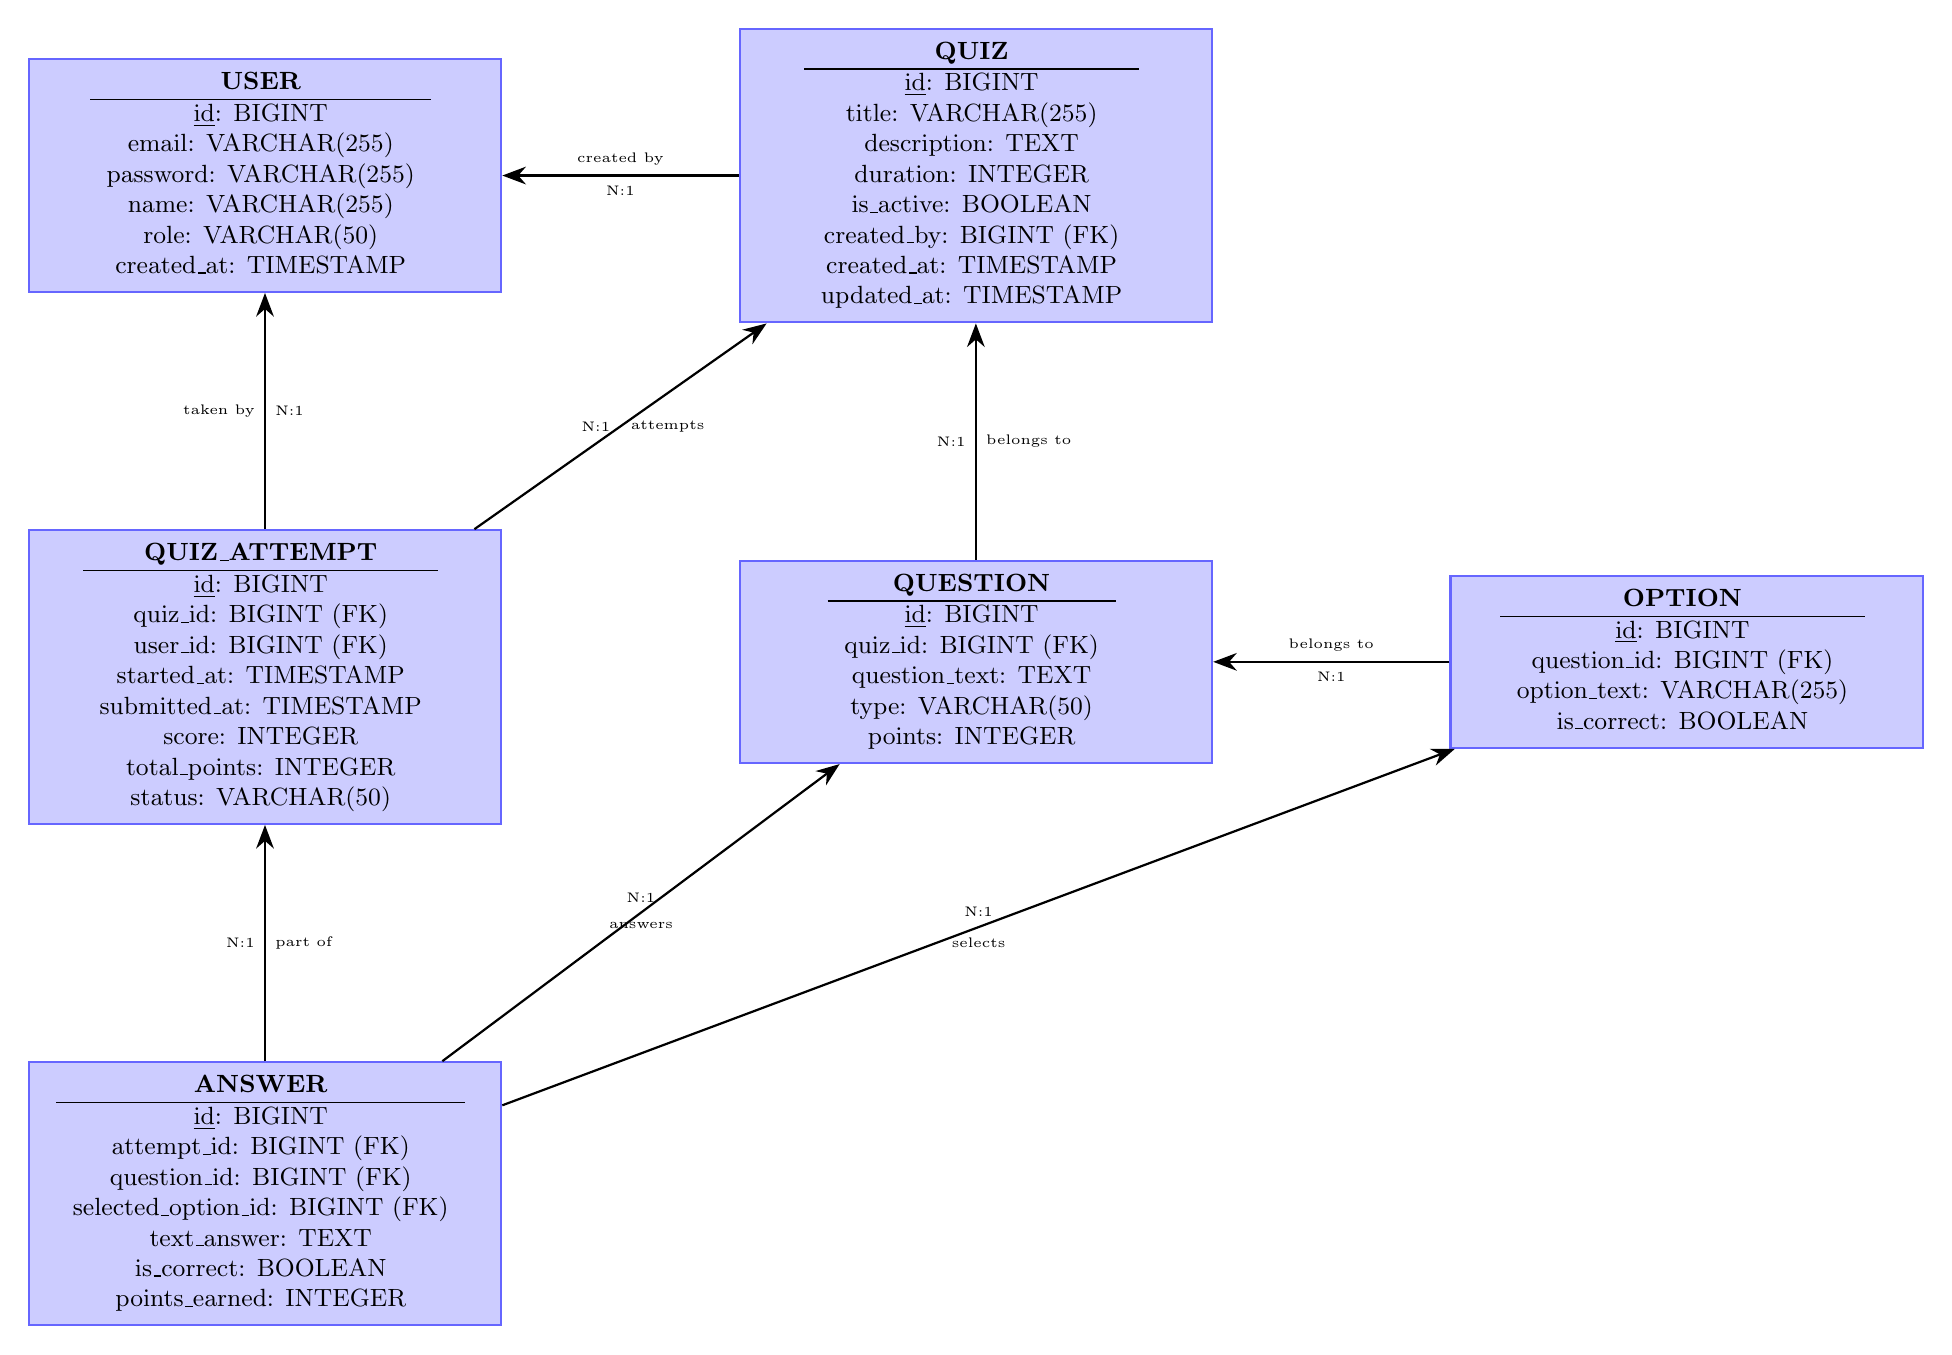
\begin{tikzpicture}[
    node distance=3cm,
    entity/.style={rectangle, draw=blue!60, fill=blue!20, thick, minimum width=6cm, align=center},
    relationship/.style={-{Stealth[length=3mm]}, thick},
    every node/.style={font=\small}
]
    
    % User Entity
    \node[entity] (user) {
        \begin{tabular}{c}
            \textbf{USER} \\
            \hline
            \underline{id}: BIGINT \\
            email: VARCHAR(255) \\
            password: VARCHAR(255) \\
            name: VARCHAR(255) \\
            role: VARCHAR(50) \\
            created\_at: TIMESTAMP
        \end{tabular}
    };
    
    % Quiz Entity
    \node[entity, right=of user] (quiz) {
        \begin{tabular}{c}
            \textbf{QUIZ} \\
            \hline
            \underline{id}: BIGINT \\
            title: VARCHAR(255) \\
            description: TEXT \\
            duration: INTEGER \\
            is\_active: BOOLEAN \\
            created\_by: BIGINT (FK) \\
            created\_at: TIMESTAMP \\
            updated\_at: TIMESTAMP
        \end{tabular}
    };
    
    % Question Entity
    \node[entity, below=of quiz] (question) {
        \begin{tabular}{c}
            \textbf{QUESTION} \\
            \hline
            \underline{id}: BIGINT \\
            quiz\_id: BIGINT (FK) \\
            question\_text: TEXT \\
            type: VARCHAR(50) \\
            points: INTEGER
        \end{tabular}
    };
    
    % Option Entity
    \node[entity, right=of question] (option) {
        \begin{tabular}{c}
            \textbf{OPTION} \\
            \hline
            \underline{id}: BIGINT \\
            question\_id: BIGINT (FK) \\
            option\_text: VARCHAR(255) \\
            is\_correct: BOOLEAN
        \end{tabular}
    };
    
    % QuizAttempt Entity
    \node[entity, below=of user] (attempt) {
        \begin{tabular}{c}
            \textbf{QUIZ\_ATTEMPT} \\
            \hline
            \underline{id}: BIGINT \\
            quiz\_id: BIGINT (FK) \\
            user\_id: BIGINT (FK) \\
            started\_at: TIMESTAMP \\
            submitted\_at: TIMESTAMP \\
            score: INTEGER \\
            total\_points: INTEGER \\
            status: VARCHAR(50)
        \end{tabular}
    };
    
    % Answer Entity
    \node[entity, below=of attempt] (answer) {
        \begin{tabular}{c}
            \textbf{ANSWER} \\
            \hline
            \underline{id}: BIGINT \\
            attempt\_id: BIGINT (FK) \\
            question\_id: BIGINT (FK) \\
            selected\_option\_id: BIGINT (FK) \\
            text\_answer: TEXT \\
            is\_correct: BOOLEAN \\
            points\_earned: INTEGER
        \end{tabular}
    };
    
    % Relationships
    \draw[relationship] (quiz) -- (user) node[midway, above, font=\tiny] {created by} node[midway, below, font=\tiny] {N:1};
    \draw[relationship] (question) -- (quiz) node[midway, right, font=\tiny] {belongs to} node[midway, left, font=\tiny] {N:1};
    \draw[relationship] (option) -- (question) node[midway, above, font=\tiny] {belongs to} node[midway, below, font=\tiny] {N:1};
    \draw[relationship] (attempt) -- (quiz) node[midway, right, font=\tiny] {attempts} node[midway, left, font=\tiny] {N:1};
    \draw[relationship] (attempt) -- (user) node[midway, left, font=\tiny] {taken by} node[midway, right, font=\tiny] {N:1};
    \draw[relationship] (answer) -- (attempt) node[midway, right, font=\tiny] {part of} node[midway, left, font=\tiny] {N:1};
    \draw[relationship] (answer) -- (question) node[midway, below, font=\tiny] {answers} node[midway, above, font=\tiny] {N:1};
    \draw[relationship] (answer) -- (option) node[midway, below, font=\tiny] {selects} node[midway, above, font=\tiny] {N:1};
    
\end{tikzpicture}
\caption{Complete Entity-Relationship Diagram}
\end{figure}
\end{landscape}

\section{Relationship Details}

\subsection{User $\rightarrow$ Quiz (created\_by)}

\begin{table}[h]
\centering
\begin{tabular}{|l|p{8cm}|}
\hline
\textbf{Type} & One-to-Many \\
\hline
\textbf{Cardinality} & 1 User : N Quizzes \\
\hline
\textbf{Direction} & Unidirectional (Quiz $\rightarrow$ User) \\
\hline
\textbf{Foreign Key} & quizzes.created\_by $\rightarrow$ users.id \\
\hline
\textbf{On Delete} & Depends on business rule (typically RESTRICT) \\
\hline
\textbf{Description} & Each quiz is created by exactly one admin user. A user (admin) can create multiple quizzes. \\
\hline
\textbf{JPA Mapping} & @ManyToOne(fetch = FetchType.LAZY) in Quiz \\
\hline
\end{tabular}
\caption{User-Quiz Relationship}
\end{table}

\textbf{SQL Constraint:}
\begin{lstlisting}[language=SQL]
ALTER TABLE quizzes
ADD CONSTRAINT fk_quiz_created_by
FOREIGN KEY (created_by) REFERENCES users(id);
\end{lstlisting}

\subsection{Quiz $\leftrightarrow$ Question}

\begin{table}[h]
\centering
\begin{tabular}{|l|p{8cm}|}
\hline
\textbf{Type} & One-to-Many (Bidirectional) \\
\hline
\textbf{Cardinality} & 1 Quiz : N Questions \\
\hline
\textbf{Foreign Key} & questions.quiz\_id $\rightarrow$ quizzes.id \\
\hline
\textbf{Cascade} & ALL (persist, merge, remove, refresh, detach) \\
\hline
\textbf{Orphan Removal} & true (delete questions if removed from list) \\
\hline
\textbf{Description} & Each question belongs to exactly one quiz. A quiz contains multiple questions. When a quiz is deleted, all its questions are automatically deleted. \\
\hline
\textbf{JPA Mapping} & @OneToMany in Quiz, @ManyToOne in Question \\
\hline
\end{tabular}
\caption{Quiz-Question Relationship}
\end{table}

\textbf{SQL Constraint:}
\begin{lstlisting}[language=SQL]
ALTER TABLE questions
ADD CONSTRAINT fk_question_quiz
FOREIGN KEY (quiz_id) REFERENCES quizzes(id)
ON DELETE CASCADE;
\end{lstlisting}

\subsection{Question $\leftrightarrow$ Option}

\begin{table}[h]
\centering
\begin{tabular}{|l|p{8cm}|}
\hline
\textbf{Type} & One-to-Many (Bidirectional) \\
\hline
\textbf{Cardinality} & 1 Question : N Options \\
\hline
\textbf{Foreign Key} & options.question\_id $\rightarrow$ questions.id \\
\hline
\textbf{Cascade} & ALL \\
\hline
\textbf{Orphan Removal} & true \\
\hline
\textbf{Description} & Each option belongs to exactly one question. A question can have multiple options (typically 4-5 for multiple choice). Options are deleted when question is deleted. \\
\hline
\textbf{JPA Mapping} & @OneToMany in Question, @ManyToOne in Option \\
\hline
\end{tabular}
\caption{Question-Option Relationship}
\end{table}

\subsection{Quiz $\rightarrow$ QuizAttempt}

\begin{table}[h]
\centering
\begin{tabular}{|l|p{8cm}|}
\hline
\textbf{Type} & One-to-Many \\
\hline
\textbf{Cardinality} & 1 Quiz : N Attempts \\
\hline
\textbf{Foreign Key} & quiz\_attempts.quiz\_id $\rightarrow$ quizzes.id \\
\hline
\textbf{Description} & Each attempt is for exactly one quiz. A quiz can have multiple attempts from different candidates. \\
\hline
\textbf{Business Rule} & Typically prevent quiz deletion if attempts exist \\
\hline
\end{tabular}
\caption{Quiz-Attempt Relationship}
\end{table}

\subsection{User $\rightarrow$ QuizAttempt}

\begin{table}[h]
\centering
\begin{tabular}{|l|p{8cm}|}
\hline
\textbf{Type} & One-to-Many \\
\hline
\textbf{Cardinality} & 1 User : N Attempts \\
\hline
\textbf{Foreign Key} & quiz\_attempts.user\_id $\rightarrow$ users.id \\
\hline
\textbf{Description} & Each attempt is taken by exactly one candidate. A candidate can take multiple quizzes and can retake the same quiz multiple times. \\
\hline
\end{tabular}
\caption{User-Attempt Relationship}
\end{table}

\subsection{QuizAttempt $\leftrightarrow$ Answer}

\begin{table}[h]
\centering
\begin{tabular}{|l|p{8cm}|}
\hline
\textbf{Type} & One-to-Many (Bidirectional) \\
\hline
\textbf{Cardinality} & 1 Attempt : N Answers \\
\hline
\textbf{Foreign Key} & answers.attempt\_id $\rightarrow$ quiz\_attempts.id \\
\hline
\textbf{Cascade} & ALL \\
\hline
\textbf{Orphan Removal} & true \\
\hline
\textbf{Description} & Each answer belongs to exactly one attempt. An attempt contains multiple answers (one per question). Answers are deleted when attempt is deleted. \\
\hline
\end{tabular}
\caption{Attempt-Answer Relationship}
\end{table}

\subsection{Question $\rightarrow$ Answer}

\begin{table}[h]
\centering
\begin{tabular}{|l|p{8cm}|}
\hline
\textbf{Type} & One-to-Many \\
\hline
\textbf{Cardinality} & 1 Question : N Answers \\
\hline
\textbf{Foreign Key} & answers.question\_id $\rightarrow$ questions.id \\
\hline
\textbf{Description} & Each answer is for exactly one question. A question can have many answers across different attempts. \\
\hline
\end{tabular}
\caption{Question-Answer Relationship}
\end{table}

\subsection{Option $\rightarrow$ Answer}

\begin{table}[h]
\centering
\begin{tabular}{|l|p{8cm}|}
\hline
\textbf{Type} & One-to-Many (Optional) \\
\hline
\textbf{Cardinality} & 1 Option : N Answers \\
\hline
\textbf{Foreign Key} & answers.selected\_option\_id $\rightarrow$ options.id (NULLABLE) \\
\hline
\textbf{Description} & For multiple-choice questions, an answer references the selected option. For short-answer questions, this field is null. An option can be selected by multiple candidates. \\
\hline
\end{tabular}
\caption{Option-Answer Relationship}
\end{table}

\section{Database Constraints}

\subsection{Primary Keys}

All tables use auto-incrementing BIGINT primary keys:
\begin{itemize}
    \item BIGSERIAL in PostgreSQL
    \item GenerationType.IDENTITY in JPA
    \item Range: -9,223,372,036,854,775,808 to 9,223,372,036,854,775,807
\end{itemize}

\subsection{Foreign Key Constraints}

\begin{table}[h]
\centering
\small
\begin{tabular}{|l|l|l|}
\hline
\textbf{Table} & \textbf{FK Column} & \textbf{References} \\
\hline
quizzes & created\_by & users(id) \\
\hline
questions & quiz\_id & quizzes(id) \\
\hline
options & question\_id & questions(id) \\
\hline
quiz\_attempts & quiz\_id & quizzes(id) \\
\hline
quiz\_attempts & user\_id & users(id) \\
\hline
answers & attempt\_id & quiz\_attempts(id) \\
\hline
answers & question\_id & questions(id) \\
\hline
answers & selected\_option\_id & options(id) \\
\hline
\end{tabular}
\caption{Foreign Key Summary}
\end{table}

\subsection{Unique Constraints}

\begin{itemize}
    \item \textbf{users.email}: Must be unique (used for authentication)
\end{itemize}

\subsection{Not Null Constraints}

Critical fields that cannot be null:
\begin{itemize}
    \item All primary keys
    \item All foreign keys (except answers.selected\_option\_id)
    \item users: email, password, name, role, created\_at
    \item quizzes: title, duration, is\_active, created\_by
    \item questions: quiz\_id, question\_text, type, points
    \item options: question\_id, option\_text, is\_correct
    \item quiz\_attempts: quiz\_id, user\_id, started\_at, status
    \item answers: attempt\_id, question\_id, is\_correct
\end{itemize}

\section{Indexes}

Recommended indexes for performance:

\begin{lstlisting}[language=SQL]
-- Email lookup for authentication
CREATE INDEX idx_users_email ON users(email);

-- Active quiz queries
CREATE INDEX idx_quizzes_is_active ON quizzes(is_active);

-- User attempt history
CREATE INDEX idx_quiz_attempts_user_id ON quiz_attempts(user_id);

-- Quiz analytics
CREATE INDEX idx_quiz_attempts_quiz_id ON quiz_attempts(quiz_id);

-- Attempt status filtering
CREATE INDEX idx_quiz_attempts_status ON quiz_attempts(status);
\end{lstlisting}



\end{document}
